\documentclass[tikz,border=3pt]{standalone}
\usepackage[utf8]{inputenc}
\usepackage[T1]{fontenc}
\usepackage{lmodern}
\renewcommand{\familydefault}{\sfdefault}
\usepackage{sansmath}\sansmath
\usepackage{chemfig}
\usepackage{pgfplots}\pgfplotsset{compat=1.18,/pgf/number format/use comma,/pgf/number format/1000 sep={.}}
\usetikzlibrary{arrows.meta,calc,positioning,decorations.pathmorphing,patterns}
% paleta del sitio
\definecolor{nar}{HTML}{E8680C}\definecolor{narc}{HTML}{FFB35C}\definecolor{hielo}{HTML}{FFF3E8}
\definecolor{tinta}{HTML}{1D1D1F}\definecolor{gris}{HTML}{6E6E73}\definecolor{lila}{HTML}{7C5CF0}
\definecolor{azul}{HTML}{2F6FD6}\definecolor{menta}{HTML}{17A673}\definecolor{coral}{HTML}{E8342A}
\begin{document}
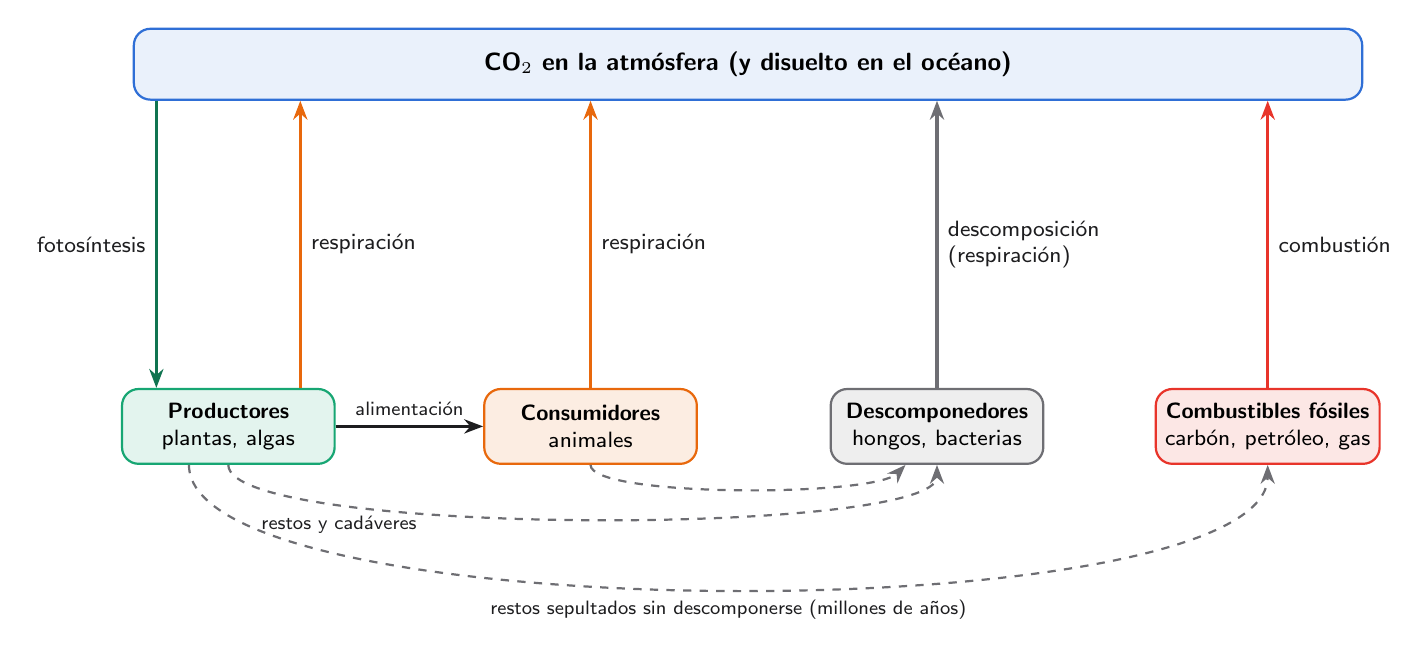
\begin{tikzpicture}[font=\footnotesize,>={Stealth[length=2.4mm]}]
\tikzset{caja/.style={draw=#1,fill=#1!12,thick,rounded corners=6pt,minimum width=2.7cm,minimum height=0.95cm,align=center,font=\footnotesize}}
\node[draw=azul,fill=azul!10,thick,rounded corners=6pt,minimum width=15.6cm,minimum height=0.9cm,font=\small\bfseries] (A) at (6.6,4.6) {CO$_2$ en la atmósfera (y disuelto en el océano)};
\node[caja=menta] (P) at (0,0) {\textbf{Productores}\\plantas, algas};
\node[caja=nar] (C) at (4.6,0) {\textbf{Consumidores}\\animales};
\node[caja=gris] (D) at (9.0,0) {\textbf{Descomponedores}\\hongos, bacterias};
\node[caja=coral] (F) at (13.2,0) {\textbf{Combustibles fósiles}\\carbón, petróleo, gas};
\draw[->,very thick,menta!70!black] (P.north west |- A.south) ++(0.45,0) -- ($(P.north west)+(0.45,0)$) node[midway,left,text=tinta] {fotosíntesis};
\draw[->,very thick,nar] ($(P.north east)+(-0.45,0)$) -- ($(P.north east |- A.south)+(-0.45,0)$) node[midway,right,text=tinta] {respiración};
\draw[->,very thick,nar] (C.north) -- (C.north |- A.south) node[midway,right,text=tinta] {respiración};
\draw[->,very thick,gris] (D.north) -- (D.north |- A.south) node[midway,right,text=tinta,align=left] {descomposición\\(respiración)};
\draw[->,very thick,coral] (F.north) -- (F.north |- A.south) node[midway,right,text=tinta] {combustión};
\draw[->,very thick,tinta] (P) -- (C) node[midway,above,font=\scriptsize] {alimentación};
\draw[->,thick,gris,dashed] (P.south) .. controls (0,-1.4) and (9,-1.4) .. (D.south) node[pos=0.25,below,text=tinta,font=\scriptsize] {restos y cadáveres};
\draw[->,thick,gris,dashed] (C.south) .. controls (4.6,-0.9) and (8.2,-0.9) .. ($(D.south)+(-0.4,0)$);
\draw[->,thick,gris,dashed] ($(P.south)+(-0.5,0)$) .. controls (-0.5,-2.6) and (13.2,-2.6) .. (F.south) node[pos=0.5,below,text=tinta,font=\scriptsize] {restos sepultados sin descomponerse (millones de años)};
\end{tikzpicture}
\end{document}
